\documentclass[aspectratio=169,9pt]{beamer}

\usepackage[T5]{fontenc}
\usepackage[utf8]{inputenc}
\usepackage[vietnamese]{babel}
\usepackage{lmodern}
\usepackage{amsmath,amssymb}
\usepackage{graphicx}
\usepackage{booktabs}
\usepackage{tabularx}
\usepackage{array}
\usepackage{ragged2e}
\usepackage{tcolorbox}

\graphicspath{{./}{assets/}}

\definecolor{PTITRed}{RGB}{166,25,31}
\definecolor{Ink}{RGB}{42,44,52}
\definecolor{Muted}{RGB}{102,108,118}
\definecolor{Line}{RGB}{188,192,200}
\definecolor{Panel}{RGB}{247,247,248}
\definecolor{PaleRed}{RGB}{249,239,240}

\setbeamertemplate{navigation symbols}{}
\setbeamertemplate{headline}{}
\setbeamersize{text margin left=0.55cm,text margin right=0.55cm}
\setbeamercolor{normal text}{fg=Ink,bg=white}
\setbeamercolor{frametitle}{fg=white,bg=PTITRed}
\setbeamercolor{itemize item}{fg=PTITRed}
\setbeamerfont{normal text}{size=\fontsize{8.9}{10.6}\selectfont}
\setbeamerfont{frametitle}{size=\fontsize{12.4}{14.4}\selectfont,series=\bfseries}
\setbeamerfont{itemize/enumerate body}{size=\fontsize{8.9}{10.6}\selectfont}
\setbeamertemplate{itemize item}{\raisebox{0.14ex}{\scriptsize$\blacktriangleright$}}
\setbeamertemplate{itemize subitem}{\raisebox{0.14ex}{\tiny$\blacktriangleright$}}
\setbeamertemplate{enumerate item}{\color{PTITRed}\insertenumlabel.}

\setbeamertemplate{frametitle}{
  \nointerlineskip
  \begin{beamercolorbox}[wd=\paperwidth,ht=0.67cm,dp=0.36cm,center]{frametitle}
    \insertframetitle
  \end{beamercolorbox}
}

\setbeamertemplate{footline}{
  \leavevmode
  \hbox to \paperwidth{\hfill
    \colorbox{PTITRed}{\makebox[0.30cm][c]{\color{white}\fontsize{5.2}{5.2}\selectfont\insertframenumber}}
    \hspace{0.46cm}}
  \vspace{0.28cm}
}

\newcommand{\smallnote}[1]{{\fontsize{7.1}{8.4}\selectfont #1\par}}
\newcommand{\tinytext}[1]{{\fontsize{6.3}{7.3}\selectfont #1\par}}
\newcommand{\heading}[1]{{\bfseries\color{PTITRed} #1\par}}
\newcommand{\numlabel}[1]{\colorbox{PTITRed}{\makebox[0.48cm][c]{\color{white}\bfseries #1}}}
\newcommand{\tightitems}{\setlength{\itemsep}{0.13em}\setlength{\parskip}{0pt}\setlength{\parsep}{0pt}}
\newcommand{\verytightitems}{\setlength{\itemsep}{0.04em}\setlength{\parskip}{0pt}\setlength{\parsep}{0pt}}

\tcbset{
  panel/.style={colback=Panel,colframe=Line,boxrule=0.42pt,arc=0.8mm,left=1.6mm,right=1.6mm,top=1.1mm,bottom=1.1mm,before skip=0pt,after skip=0pt},
  keypanel/.style={colback=PaleRed,colframe=PTITRed,boxrule=0.55pt,arc=0.8mm,left=1.7mm,right=1.7mm,top=1.1mm,bottom=1.1mm,before skip=0pt,after skip=0pt},
  titlepanel/.style={colback=white,colframe=Line,boxrule=0.45pt,arc=0mm,left=1.5mm,right=1.5mm,top=0.5mm,bottom=1.1mm,fonttitle=\bfseries,coltitle=white,colbacktitle=PTITRed,titlerule=0pt},
  equalpanel/.style={colback=white,colframe=Line,boxrule=0.45pt,arc=0mm,left=1.6mm,right=1.6mm,top=1.3mm,bottom=1.3mm,height=4.40cm,valign=top}
}

\newcolumntype{L}[1]{>{\RaggedRight\arraybackslash}p{#1}}
\newcolumntype{R}[1]{>{\RaggedLeft\arraybackslash}p{#1}}
\newcolumntype{C}[1]{>{\Centering\arraybackslash}p{#1}}
\newcolumntype{Y}{>{\RaggedRight\arraybackslash}X}


\usepackage{tikz}
\usetikzlibrary{positioning}
\newcommand{\srcn}[1]{{\fontsize{7.0}{8.2}\selectfont\color{Muted}Nguồn: #1}}
\newcommand{\kpi}[2]{\begin{tcolorbox}[panel]\centering{\color{PTITRed}\bfseries\fontsize{18}{19}\selectfont #1\par}\vspace{0.04cm}\smallnote{#2}\end{tcolorbox}}

\begin{document}

% ---------- 01: Cover ----------
\begin{frame}[plain]
\centering\vspace{0.12cm}
{\color{PTITRed}\bfseries\fontsize{12.2}{14}\selectfont HỌC VIỆN CÔNG NGHỆ BƯU CHÍNH VIỄN THÔNG\par}
\vspace{0.08cm}{\fontsize{8.5}{10}\selectfont Khoa Kĩ thuật Điện tử 1\par}
\vspace{0.20cm}{\color{PTITRed}\rule{0.76\linewidth}{0.75pt}\par}
\vspace{0.36cm}
{\color{PTITRed}\bfseries\fontsize{17}{20}\selectfont BÁO CÁO TIẾN ĐỘ NGHIÊN CỨU\par}
\vspace{0.24cm}
{\bfseries\fontsize{14.5}{17}\selectfont VideoMamba-Tiny trên CTPGesture v1\par}
\vspace{0.10cm}
{\fontsize{9.8}{11.5}\selectfont Isolated Gesture Classification, Continuous Recognition\\
và đối chiếu các công trình liên quan\par}
\vspace{0.48cm}
{\fontsize{8.4}{10}\selectfont
\begin{tabular}{@{}l@{\hspace{0.5cm}}l@{}}
\textcolor{PTITRed}{\bfseries Sinh viên:}& Nguyễn Hữu Hoàng Anh\\[0.1cm]
\textcolor{PTITRed}{\bfseries Lĩnh vực:}& Video Action / Gesture Recognition\\[0.1cm]
\textcolor{PTITRed}{\bfseries Đầu vào:}& RGB video, CTPGesture v1 (9 lớp)
\end{tabular}\par}
\vfill
{\color{Muted}\fontsize{7.9}{9}\selectfont Hà Nội, ngày 15 tháng 10 năm 2026\par}
\end{frame}

% ---------- 02: Outline ----------
\begin{frame}{Nội dung báo cáo}
\vspace{0.18cm}
\renewcommand{\arraystretch}{1.68}
\begin{tabularx}{\linewidth}{@{}C{0.7cm}L{3.55cm}Y@{}}
\toprule
\textbf{STT}&\textbf{Nhóm nội dung}&\textbf{Trọng tâm}\\\midrule
1&\textcolor{PTITRed}{\bfseries Thiết lập}&Dataset, checkpoint, đánh giá isolated / continuous.\\
2&\textcolor{PTITRed}{\bfseries Thực nghiệm}&Accuracy, Macro-F1, confusion matrices, post-processing.\\
3&\textcolor{PTITRed}{\bfseries Hiệu năng}&Parameters, estimated GFLOPs, latency, throughput.\\
4&\textcolor{PTITRed}{\bfseries Bốn bài đối chứng}&Venue, phương pháp, bằng chứng Table/Page, khác protocol.\\
5&\textcolor{PTITRed}{\bfseries Hướng tiếp theo}&Fair causal benchmark và phân đoạn chuỗi hành động.\\\bottomrule
\end{tabularx}
\vspace{0.23cm}
\begin{tcolorbox}[keypanel]\centering
\bfseries Phân biệt kết quả nhận dạng đoạn đã biết ranh giới và kết quả nhận dạng trên toàn bộ video.
\end{tcolorbox}
\end{frame}

% ---------- 03: Dataset ----------
\begin{frame}{1. Dataset CTPGesture v1 và kiểm kê test set}
\begin{columns}[T,onlytextwidth]
\begin{column}{0.50\textwidth}
\begin{tcolorbox}[titlepanel,title=Dữ liệu đầu vào,height=4.7cm]
\begin{itemize}\tightitems
\item Video RGB, nhãn \textbf{theo từng frame}.
\item \textbf{9 lớp}: 8 lệnh giao thông và No Gesture.
\item Frame rate: \textbf{15 FPS}.
\item Test audit trong notebook: \textbf{11 video}.
\item Tổng cộng \textbf{67.356 frames}.
\end{itemize}
\end{tcolorbox}
\end{column}
\begin{column}{0.48\textwidth}
\begin{tcolorbox}[titlepanel,title=Đơn vị đánh giá,height=4.7cm]
\centering\vspace{0.08cm}
{\fontsize{19}{21}\selectfont\color{PTITRed}\bfseries 1.728\par}
\smallnote{Temporal segments}\vspace{0.19cm}
{\fontsize{15}{17}\selectfont\bfseries 869 / 859\par}
\smallnote{No Gesture / Gesture}\vspace{0.19cm}
\smallnote{\textbf{Test video IDs}:\\002, 004, 008, 010, 012, 014, 016, 018, 101, 102, 104}
\end{tcolorbox}
\end{column}
\end{columns}
\vspace{0.08cm}\srcn{Notebook Cell 10: OFFICIAL CTPGesture TEST SPLIT.}
\end{frame}

% ---------- 04: Pipeline ----------
\begin{frame}{1. Pipeline VideoMamba-Tiny và hai giao thức}
\vspace{0.08cm}
\begin{center}
\begin{tikzpicture}[every node/.style={font=\fontsize{8}{9}\selectfont}]
\node[draw=Line,fill=Panel,rounded corners=2pt,minimum height=0.82cm,text width=2.3cm,align=center] (a) {RGB video\\15 FPS};
\node[draw=Line,fill=Panel,rounded corners=2pt,minimum height=0.82cm,text width=2.3cm,align=center,right=0.55cm of a] (b) {16 sampled frames\\$224\times224$};
\node[draw=Line,fill=Panel,rounded corners=2pt,minimum height=0.82cm,text width=2.3cm,align=center,right=0.55cm of b] (c) {VideoMamba-Tiny\\Selective SSM};
\node[draw=Line,fill=Panel,rounded corners=2pt,minimum height=0.82cm,text width=2.3cm,align=center,right=0.55cm of c] (d) {Class probabilities\\9 labels};
\draw[-stealth,thick,PTITRed] (a)--(b);\draw[-stealth,thick,PTITRed] (b)--(c);\draw[-stealth,thick,PTITRed] (c)--(d);
\end{tikzpicture}
\end{center}
\vspace{0.18cm}
\begin{columns}[T,onlytextwidth]
\begin{column}{0.49\textwidth}
\begin{tcolorbox}[panel]
\heading{A. Isolated classification}
\begin{itemize}\tightitems
\item Ground-truth boundaries tạo clip.
\item Lấy 16 frame đều trong mỗi segment.
\item 1 dự đoán / segment.
\item Báo cáo Accuracy và Macro-F1.
\end{itemize}
\end{tcolorbox}
\end{column}
\begin{column}{0.49\textwidth}
\begin{tcolorbox}[panel]
\heading{B. Continuous recognition}
\begin{itemize}\tightitems
\item Window \textbf{32 frames}, step \textbf{8 frames}.
\item Overlap \textbf{75\%}; sample 16 frames.
\item Tổng hợp xác suất các cửa sổ lên frame.
\item Không phải phép dự đoán causal thuần.
\end{itemize}
\end{tcolorbox}
\end{column}
\end{columns}
\vspace{0.05cm}\srcn{Notebook Cells 13--18, 22.}
\end{frame}

% ---------- 05: Setup ----------
\begin{frame}{1. Cấu hình thử nghiệm được lưu trong notebook}
\vspace{0.02cm}
{\fontsize{8.2}{9.5}\selectfont
\renewcommand{\arraystretch}{1.16}
\begin{tabularx}{\linewidth}{@{}L{3.9cm}Y L{3cm}@{}}
\toprule
\textbf{Thành phần}&\textbf{Thiết lập}&\textbf{Ghi chú}\\\midrule
Model & VideoMamba-Tiny & 24 layers\\
Weights & \texttt{checkpoint-best.pth} & Epoch 17\\
Input tensor & $[B,3,16,224,224]$ & FP32\\
Số lớp & 9 & No Gesture + 8 gestures\\
Window / step & 32 / 8 frames & 2,13 s / 0,53 s @15 FPS\\
Sample offsets & $0,2,4,\ldots,30$ & 16 frames mỗi window\\
Inference GPU & NVIDIA Tesla T4 & \texttt{native\_cuda}\\
Evaluation batch & 4 & Isolated và continuous\\
Runtime benchmark batch & 1 & Đo model-only latency\\\bottomrule
\end{tabularx}
}
\vspace{0.08cm}
\srcn{Notebook Cells 6, 8, 10, 26. Training hyperparameters cần bổ sung từ notebook huấn luyện.}
\end{frame}

% ---------- 06: Isolated ----------
\begin{frame}{2. Isolated Classification -- kết quả 9 lớp}
\begin{columns}[T,onlytextwidth]
\begin{column}{0.51\textwidth}
\begin{columns}[T,onlytextwidth]
\begin{column}{0.49\textwidth}\kpi{98,55\%}{Top-1 Accuracy\\1.728 segments}\end{column}
\begin{column}{0.49\textwidth}\kpi{97,96\%}{Macro-F1\\9 classes}\end{column}
\end{columns}
\vspace{0.13cm}
\begin{tcolorbox}[panel]
\heading{Gesture-only (GT lớp 1--8)}
\begin{itemize}\tightitems
\item \textbf{859} gesture segments.
\item Accuracy: \textbf{98,02\%}.
\item Macro-F1: \textbf{98,24\%}.
\item Balanced Accuracy (9 lớp): 98,12\%.
\end{itemize}
\end{tcolorbox}
\smallnote{\textbf{Diễn giải:} Phân loại chính xác cao khi \emph{đã biết trước} ranh giới cử chỉ.}
\end{column}
\begin{column}{0.46\textwidth}
\centering
\IfFileExists{cell17_output5.png}{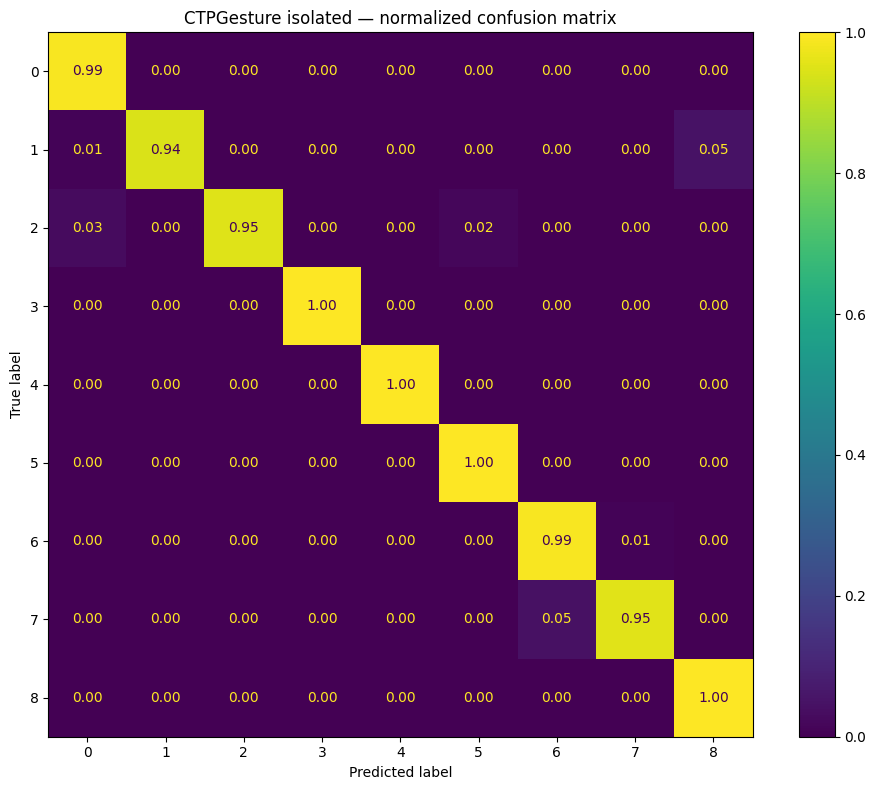
\includegraphics[height=5.05cm,keepaspectratio]{cell17_output5.png}}{\begin{tcolorbox}[panel]Thiếu ảnh confusion matrix\end{tcolorbox}}
\tinytext{Confusion matrix -- isolated}
\end{column}
\end{columns}
\vspace{0.04cm}\srcn{Notebook Cell 16, ảnh \texttt{cell17\_output5.png}.}
\end{frame}

% ---------- 07: Continuous ----------
\begin{frame}{2. Continuous Recognition -- RAW, toàn bộ test video}
\begin{columns}[T,onlytextwidth]
\begin{column}{0.51\textwidth}
\begin{columns}[T,onlytextwidth]
\begin{column}{0.49\textwidth}\kpi{83,98\%}{Global Frame Accuracy}\end{column}
\begin{column}{0.49\textwidth}\kpi{80,61\%}{Global Macro-F1}\end{column}
\end{columns}
\vspace{0.13cm}
\begin{tcolorbox}[panel]
\heading{Thiết lập và temporal metrics}
\begin{itemize}\tightitems
\item 11 videos / \textbf{67.356 frames}.
\item \textbf{8.392} windows (32/8).
\item Mean Gesture Recall: \textbf{94,80\%}.
\item Mean Temporal Overlap: \textbf{65,32\%}.
\end{itemize}
\end{tcolorbox}
\smallnote{\textbf{Vấn đề:} Hiệu năng giảm ở bài toán liên tục, cần kiểm tra transitions và temporal boundaries.}
\end{column}
\begin{column}{0.46\textwidth}
\centering
\IfFileExists{cell23_output5.png}{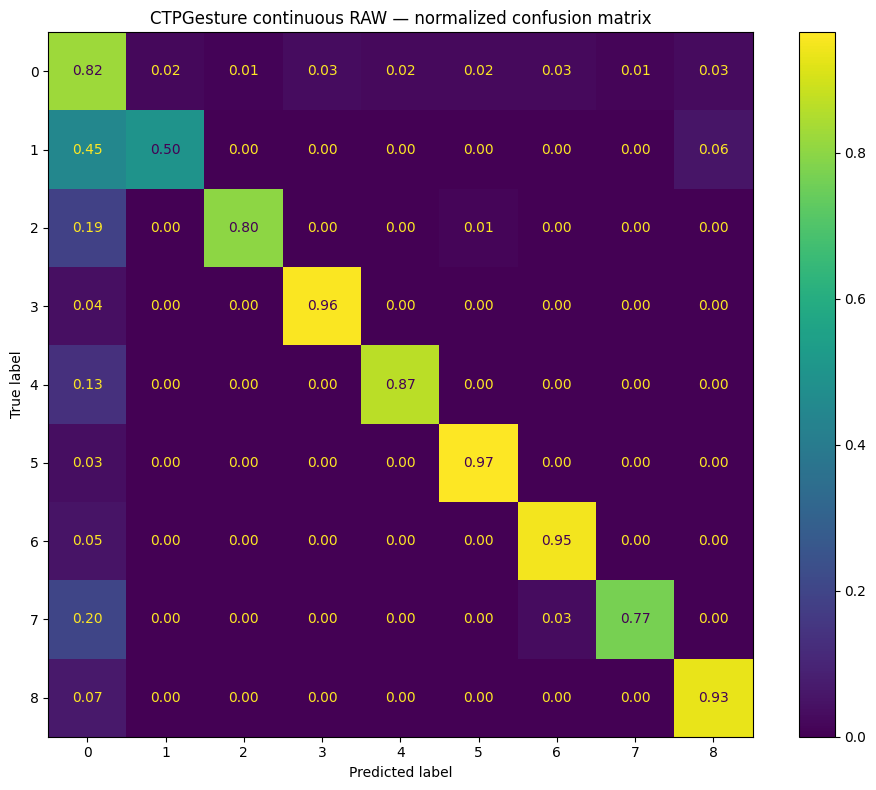
\includegraphics[height=5.05cm,keepaspectratio]{cell23_output5.png}}{\begin{tcolorbox}[panel]Thiếu ảnh confusion matrix\end{tcolorbox}}
\tinytext{Confusion matrix -- continuous RAW}
\end{column}
\end{columns}
\vspace{0.04cm}\srcn{Notebook Cell 22, ảnh \texttt{cell23\_output5.png}.}
\end{frame}

% ---------- 08: Postprocessing ----------
\begin{frame}{2. Hậu xử lí -- hiệu quả và giới hạn suy luận}
\vspace{0.04cm}
\renewcommand{\arraystretch}{1.44}
\begin{tabularx}{\linewidth}{@{}L{4cm}C{2.35cm}C{2.35cm}Y@{}}
\toprule
\textbf{Cấu hình}&\textbf{Frame Acc.}&\textbf{Macro-F1}&\textbf{Temporal overlap}\\\midrule
RAW, không hậu xử lí & 83,98\% & 80,61\% & 65,32\%\\
R3, loại đoạn ngắn dưới 1 s & \textbf{83,99\%} & \textbf{80,63\%} & \textbf{65,90\%}\\
S1, smoothing & 83,81\% & 79,71\% & 64,85\%\\\bottomrule
\end{tabularx}
\vspace{0.20cm}
\begin{columns}[T,onlytextwidth]
\begin{column}{0.49\textwidth}
\begin{tcolorbox}[panel]
\heading{Quan sát}
\begin{itemize}\tightitems
\item R3 tăng overlap 0,58 điểm \%.
\item Frame Accuracy tăng rất nhỏ.
\item Probability smoothing làm giảm Macro-F1.
\end{itemize}
\end{tcolorbox}
\end{column}
\begin{column}{0.49\textwidth}
\begin{tcolorbox}[keypanel]
\heading{Giới hạn methodology}
\smallnote{R3 được chọn khi thử các cấu hình trên \textbf{test set}. Do vậy R3 chỉ có ý nghĩa thăm dò; báo cáo \textbf{RAW} là kết quả chính cho đến khi tune trên validation.}
\end{tcolorbox}
\end{column}
\end{columns}
\vspace{0.04cm}\srcn{Notebook Cell 24: post-processing ablation.}
\end{frame}

% ---------- 09: Complexity ----------
\begin{frame}{3. Model Complexity và Runtime (NVIDIA Tesla T4)}
\vspace{0.01cm}
\begin{columns}[T,onlytextwidth]
\begin{column}{0.24\textwidth}\kpi{6,96M}{Parameters}\end{column}
\begin{column}{0.24\textwidth}\kpi{29,03}{Estimated GFLOPs/clip}\end{column}
\begin{column}{0.24\textwidth}\kpi{50,65}{ms/clip, batch 1}\end{column}
\begin{column}{0.24\textwidth}\kpi{19,74}{clips/s, batch 1}\end{column}
\end{columns}
\vspace{0.09cm}
\renewcommand{\arraystretch}{1.24}
\begin{tabularx}{\linewidth}{@{}L{3.9cm}X L{2.6cm}@{}}
\toprule
\textbf{Phép đo}&\textbf{Kết quả}&\textbf{Điều kiện}\\\midrule
Mean / median / p95 latency & 50,65 / 50,79 / 51,00 ms & Batch=1, FP32\\
Continuous model forward & 48,17 ms/window & Batch=4\\
Full-test wall time & 968,01 s / 8.392 windows & 11 videos\\
Effective throughput & 8,67 windows/s & Full evaluation loop\\
Extra GPU allocation & 56,58 MiB & Không phải peak VRAM tổng\\\bottomrule
\end{tabularx}
\vspace{0.10cm}
\srcn{Notebook Cells 22, 26. 29,03 GFLOPs là \textbf{ước lượng custom counter}, cần kiểm tra quy ước MAC/FLOP.}
\end{frame}

% ---------- 10: Realtime ----------
\begin{frame}{3. Giải thích số đo latency và khả năng real-time}
\begin{columns}[T,onlytextwidth]
\begin{column}{0.49\textwidth}
\begin{tcolorbox}[titlepanel,title=Những gì đã đo,height=4.5cm]
\begin{itemize}\tightitems
\item \textbf{50,65 ms}: chạy 1 clip / model forward, FP32, Tesla T4.
\item \textbf{8,67 windows/s}: throughput của phép đánh giá offline, có decode.
\item 1 window gồm 32 frames (2,13 s ở 15 FPS).
\item Bước dịch window: 8 frames (0,53 s).
\end{itemize}
\end{tcolorbox}
\end{column}
\begin{column}{0.49\textwidth}
\begin{tcolorbox}[titlepanel,title=Những gì chưa đo,height=4.5cm]
\begin{itemize}\tightitems
\item End-to-end latency trên luồng camera.
\item Tốc độ và bộ nhớ trên Jetson/thiết bị biên.
\item Delay xuất lệnh causal theo frame.
\item Tổng peak GPU memory và mean$\pm$std qua nhiều seeds.
\end{itemize}
\end{tcolorbox}
\end{column}
\end{columns}
\vspace{0.10cm}
\begin{tcolorbox}[keypanel]\centering
\smallnote{\textbf{Không được suy ra 19,74 clips/s là 19,74 camera FPS.} Cách gán xác suất từ cửa sổ chồng lấn có thể dùng frame tương lai với một số frame đích.}
\end{tcolorbox}
\end{frame}

% ---------- 11: Literature venues ----------
\begin{frame}{4. Bốn công trình đối chứng: nơi công bố}
\vspace{0.07cm}
\renewcommand{\arraystretch}{1.55}
\begin{tabularx}{\linewidth}{@{}C{0.54cm}L{3.95cm}L{3.4cm}Y@{}}
\toprule
\textbf{ID}&\textbf{Bài báo}&\textbf{Venue / Năm}&\textbf{Ranking / trạng thái}\\\midrule
P1&Xiong et al. -- MD-GCN&Electronics, 2021&JCR 2025 Q2 (Engineering, EEE)\\
P2&Xiao et al. -- NTPGR&Scientific Reports, 2025&JCR 2025 Q1 (Multidisciplinary)\\
P3&Zhang et al. -- BiLSTM--Transformer&Electronics, 2026&JCR 2025 Q2 (Engineering, EEE)\\
P4&Li et al. -- RSC-GestureNet&arXiv preprint, 2026&Không gán quartile/CORE\\\bottomrule
\end{tabularx}
\vspace{0.16cm}
\begin{tcolorbox}[keypanel]
\smallnote{Quartile áp dụng cho \textbf{tạp chí} trong một \textbf{ngành và năm cụ thể}, không phản ánh mức trích dẫn của bài báo. Thông tin PRCV Oral của P4 do tác giả tự ghi, chưa đối chiếu proceedings.}
\end{tcolorbox}
\vspace{0.05cm}\srcn{Bốn PDF trong thư mục 261015; Electronics Journal Statistics (MDPI), số JCR 2025.}
\end{frame}

% ---------- 12: Methods P1/P2 ----------
\begin{frame}{4. Phương pháp đối chứng: Xiong (2021) và Xiao (2025)}
\begin{columns}[T,onlytextwidth]
\begin{column}{0.49\textwidth}
\begin{tcolorbox}[titlepanel,title=P1 -- MD-GCN (2021),height=5.45cm]
\smallnote{\textbf{Input / Model:} Gesture Skeleton Extractor rồi Multichannel Dilated Graph CNN, học quan hệ khớp theo không gian và thời gian.}
\vspace{0.18cm}
\smallnote{\textbf{Published:} MD-GCN \textbf{98,95\%}; các baseline RGB P3D \textbf{92,21\%}, C3D \textbf{87,12\%}.}
\vspace{0.18cm}
\smallnote{\textbf{Vị trí:} Section 6.1 (11 video train, 9 video test); \textbf{Table 3, trang 12} (Accuracy).}
\vspace{0.18cm}
\smallnote{\textbf{Lưu ý:} C3D/P3D là kết quả P1 đánh giá lại, không phải kết quả dataset trong bài C3D/P3D gốc.}
\end{tcolorbox}
\end{column}
\begin{column}{0.49\textwidth}
\begin{tcolorbox}[titlepanel,title=P2 -- NTPGR (2025),height=5.45cm]
\smallnote{\textbf{Input / Model:} EPFFNet lấy skeleton; MSNet kết hợp CNN, LSTM và temporal/channel attention.}
\vspace{0.18cm}
\smallnote{\textbf{Published:} \textbf{97,56\% Accuracy}; 759/778 cử chỉ nhận dạng đúng; response time 0,76 s.}
\vspace{0.18cm}
\smallnote{\textbf{Vị trí:} \textbf{Table 2, trang 11}; Tables 3--4, trang 13--14.}
\vspace{0.18cm}
\smallnote{\textbf{Lưu ý:} 10 test videos / 778 gesture instances; không đồng nhất split 11 videos của notebook.}
\end{tcolorbox}
\end{column}
\end{columns}
\vspace{0.05cm}\srcn{P1: electronics-10-00551-v2.pdf; P2: s41598-025-02833-y.pdf.}
\end{frame}

% ---------- 13: Methods P3/P4 ----------
\begin{frame}{4. Phương pháp đối chứng: Zhang (2026) và Li (2026)}
\begin{columns}[T,onlytextwidth]
\begin{column}{0.49\textwidth}
\begin{tcolorbox}[titlepanel,title=P3 -- BiLSTM--Transformer (2026),height=5.45cm]
\smallnote{\textbf{Input / Model:} YOLOv11m-Pose (17 keypoints), chuỗi \textbf{40 frames}, BiLSTM kết hợp Transformer.}
\vspace{0.18cm}
\smallnote{\textbf{Published:} \textbf{98,91\% Accuracy}, F1=98,91\%.}
\vspace{0.18cm}
\smallnote{\textbf{Vị trí:} Table 1 (test 10 videos); \textbf{Tables 2--4, trang 16--19}.}
\vspace{0.18cm}
\smallnote{\textbf{Cảnh báo:} Table 3 ghi BiLSTM 96,48\%, đoạn diễn giải không nhất quán; thời gian suy luận bỏ qua chi phí pose extractor.}
\end{tcolorbox}
\end{column}
\begin{column}{0.49\textwidth}
\begin{tcolorbox}[titlepanel,title=P4 -- RSC-GestureNet (2026),height=5.45cm]
\smallnote{\textbf{Input / Model:} Reliability-aware pose features, graph reasoning, pose--RGB fusion và causal temporal recognition.}
\vspace{0.18cm}
\smallnote{\textbf{Published:} \textbf{93,33$\pm$0,24\% Accuracy}; \textbf{91,71$\pm$0,27\% Macro-F1}.}
\vspace{0.18cm}
\smallnote{\textbf{Vị trí:} Section 4.1, \textbf{Table 1 trang 9}: official CTPGesture v1, causal window 32/4, trung bình 3 seeds.}
\vspace{0.18cm}
\smallnote{\textbf{Vai trò:} Đối chứng gần nhất cho continuous nhưng hiện vẫn khác cách suy luận.}
\end{tcolorbox}
\end{column}
\end{columns}
\vspace{0.05cm}\srcn{P3: electronics-15-02578.pdf; P4: 2608.02200v1.pdf.}
\end{frame}

% ---------- 14: Evidence ----------
\begin{frame}{4. Evidence matrix: số liệu trích từ đâu?}
\vspace{0.06cm}
\renewcommand{\arraystretch}{1.44}
\begin{tabularx}{\linewidth}{@{}C{0.65cm}L{3.5cm}L{3.4cm}Y@{}}
\toprule
\textbf{ID}&\textbf{Chỉ số công bố}&\textbf{Bằng chứng}&\textbf{Đơn vị / split}\\\midrule
P1&C3D 87,12\%; P3D 92,21\%; MD-GCN 98,95\%&\textbf{Table 3, PDF trang 12}&Clip-level, 9 video test\\
P2&NTPGR \textbf{97,56\%}&\textbf{Table 2, PDF trang 11}&Gesture-instance, 778 samples\\
P3&BiLSTM--Transformer \textbf{98,91\%}&\textbf{Tables 2--4, trang 16--19}&Pose sequence, 10 video test\\
P4&RSC \textbf{93,33\% Acc}; \textbf{91,71\% Macro-F1}&\textbf{Table 1, PDF trang 9}&Causal-frame, official split, 3 seeds\\\bottomrule
\end{tabularx}
\vspace{0.20cm}
\begin{tcolorbox}[keypanel]\centering
\smallnote{\textbf{Không gộp các giá trị Accuracy thành một leaderboard duy nhất:} clip classification, gesture-instance recognition và frame-level causal evaluation đo các nhiệm vụ khác nhau.}
\end{tcolorbox}
\end{frame}

% ---------- 15: Isolated comparison ----------
\begin{frame}{4. Isolated: published results dưới các protocol khác nhau}
\vspace{0.04cm}
\renewcommand{\arraystretch}{1.35}
\begin{tabularx}{\linewidth}{@{}L{3.8cm}L{2.7cm}C{2.0cm}Y@{}}
\toprule
\textbf{Model}&\textbf{Modality}&\textbf{Accuracy}&\textbf{Bối cảnh}\\\midrule
3D ResNet (P1 re-eval.) & RGB video & 81,16\% & P1 Table 3, 9 test videos\\
C3D (P1 re-eval.) & RGB video & 87,12\% & P1 Table 3, 9 test videos\\
P3D (P1 re-eval.) & RGB video & 92,21\% & P1 Table 3, 9 test videos\\
MD-GCN (P1) & Skeleton & 98,95\% & P1 Table 3, 9 test videos\\
NTPGR (P2) & Skeleton + temporal & 97,56\% & P2 Table 2, 778 gestures\\
BiLSTM--Transformer (P3) & Skeleton + temporal & 98,91\% & P3 Table 2, 10 videos\\
\textbf{VideoMamba-Tiny (ours)} & \textbf{RGB video} & \textbf{98,55\%} & \textbf{11 videos, 1.728 segments, 9 classes}\\\bottomrule
\end{tabularx}
\vspace{0.11cm}
\smallnote{\textbf{Đây là bảng đối chiếu literature, không phải fair SOTA.} Kết quả gesture-only của nhóm: 98,02\% trên 859 segments với GT labels 1--8.}
\end{frame}

% ---------- 16: Continuous comparison ----------
\begin{frame}{4. Continuous: đặt cạnh causal benchmark của P4}
\vspace{0.04cm}
\renewcommand{\arraystretch}{1.4}
\begin{tabularx}{\linewidth}{@{}L{4.05cm}C{2.15cm}C{2.15cm}Y@{}}
\toprule
\textbf{Model}&\textbf{Frame Acc.}&\textbf{Macro-F1}&\textbf{Protocol}\\\midrule
GRU (P4 reimplementation)&88,82\%&87,10\%&Causal 32/4\\
TCN (P4 reimplementation)&89,88\%&88,29\%&Causal 32/4\\
MD-GCN (P4 reimplementation)&90,08\%&88,48\%&Causal 32/4\\
RSC-GestureNet (P4)&\textbf{93,33\%}&\textbf{91,71\%}&Causal 32/4, 3 seeds\\
\textbf{VideoMamba-Tiny RAW (ours)}&\textbf{83,98\%}&\textbf{80,61\%}&Window 32/8, overlap aggregation\\\bottomrule
\end{tabularx}
\vspace{0.16cm}
\begin{tcolorbox}[keypanel]
\smallnote{\textbf{Ranh giới so sánh:} P4 gán nhãn theo quá khứ (causal). Notebook cộng xác suất từ các cửa sổ phủ lên frame nên có thể sử dụng frame tương lai. P4 báo cáo mean$\pm$std qua ba seed; notebook mới có một checkpoint.}
\end{tcolorbox}
\vspace{0.05cm}\srcn{P4 Table 1 (trang 9); notebook Cell 22.}
\end{frame}

% ---------- 17: Risks ----------
\begin{frame}{5. Những gì đã chứng minh và các hạn chế}
\begin{columns}[T,onlytextwidth]
\begin{column}{0.49\textwidth}
\begin{tcolorbox}[titlepanel,title=Kết quả đã có,height=4.65cm]
\begin{itemize}\tightitems
\item RGB end-to-end; không cần skeleton extractor.
\item Isolated: \textbf{98,55\%} Accuracy, \textbf{97,96\%} Macro-F1.
\item Continuous RAW: \textbf{83,98\%} FrameAcc, \textbf{80,61\%} Macro-F1.
\item \textbf{6,96M} params, \textbf{50,65 ms/clip} trên T4.
\item Có nguồn Table/Page cho bốn bài đối chứng.
\end{itemize}
\end{tcolorbox}
\end{column}
\begin{column}{0.49\textwidth}
\begin{tcolorbox}[titlepanel,title=Chưa đủ bằng chứng,height=4.65cm]
\begin{itemize}\tightitems
\item Cùng tên dataset nhưng khác test split/metric.
\item Chưa phải inference causal end-to-end.
\item GFLOPs mới là custom estimate.
\item Chưa có multi-seed, Edit Score và Segmental F1.
\item Chưa tách được đóng góp mới so với VideoMamba-Tiny gốc bằng ablation.
\end{itemize}
\end{tcolorbox}
\end{column}
\end{columns}
\vspace{0.15cm}
\smallnote{\textbf{Ý nghĩa:} Sự chênh lệch isolated / continuous chỉ ra yêu cầu cải thiện temporal transition, boundary modeling và protocol đánh giá.}
\end{frame}

% ---------- 18: Roadmap ----------
\begin{frame}{5. Kế hoạch thực nghiệm tiếp theo}
\vspace{0.04cm}
\renewcommand{\arraystretch}{1.52}
\begin{tabularx}{\linewidth}{@{}C{0.7cm}L{4.1cm}Y@{}}
\toprule
\textbf{P}&\textbf{Đầu việc}&\textbf{Kết quả cần bàn giao}\\\midrule
P0&Validation split riêng từ train&Không tune R3/post-processing trên official test.\\
P0&Causal end-aligned VideoMamba&Đánh giá 32/4, không dùng future frames, cùng metric P4.\\
P1&Temporal segmentation metrics&Edit Score, Segmental F1@10/25/50, per-class F1.\\
P1&Multi-seed experiments&Mean$\pm$std từ tối thiểu ba seeds.\\
P1&Đánh giá efficiency chuẩn&Xác thực GFLOPs, peak VRAM, streaming latency.\\
P2&So sánh cùng RGB modality&Triển khai lại P3D/C3D trên cùng video split.\\
P2&Ablation cho đề xuất&Chỉ rõ modification mới và đóng góp so với backbone gốc.\\\bottomrule
\end{tabularx}
\vspace{0.14cm}
\begin{tcolorbox}[keypanel]\centering
\smallnote{\textbf{Ưu tiên:} Causal protocol chung với RSC-GestureNet, sau đó bổ sung thí nghiệm so sánh công bằng.}
\end{tcolorbox}
\end{frame}

% ---------- 19: References ----------
\begin{frame}{Kết luận và danh mục tài liệu}
\begin{tcolorbox}[keypanel]\centering
{\bfseries\fontsize{12}{14}\selectfont Đánh giá bước đầu trên CTPGesture v1\par}
\vspace{0.10cm}
\smallnote{VideoMamba-Tiny đạt \textbf{98,55\% isolated Accuracy} và \textbf{83,98\% continuous Frame Accuracy}; các kết quả literature được đối chiếu theo nguồn, không suy diễn thành bảng SOTA chung protocol.}
\end{tcolorbox}
\vspace{0.14cm}
\smallnote{\textbf{Bốn công trình có PDF trong thư mục báo cáo:}}\par\vspace{0.08cm}
\tinytext{[P1] Xiong et al., \emph{Electronics} (2021), DOI: 10.3390/electronics10050551 -- Table 3.}\par\vspace{0.07cm}
\tinytext{[P2] Xiao et al., \emph{Scientific Reports} (2025), DOI: 10.1038/s41598-025-02833-y -- Table 2.}\par\vspace{0.07cm}
\tinytext{[P3] Zhang et al., \emph{Electronics} (2026), DOI: 10.3390/electronics15122578 -- Tables 2--4.}\par\vspace{0.07cm}
\tinytext{[P4] Li et al., arXiv:2608.02200v1 (2026) -- Table 1.}\par
\vspace{0.20cm}
\begin{tcolorbox}[panel]
\smallnote{\textbf{Tài liệu, notebook và nguồn kết quả:}\\
\url{https://github.com/HoangAnh301194/Research-notes/tree/main/Research_Report/261015}}
\end{tcolorbox}
\end{frame}

\end{document}
